% Python 的字符串与文件读写

\pentry{Python 入门\upref{Python}}
学习处理文件和保存数据可让你的程序使用起来更容易: 用户将能够选择输入什么样的数据, 以及在什么时候输入; 用户使用你的程序做一些工作后, 可将程序关闭, 以后再接着往下做.
\subsection{Python文件读写的方法}
\textbf{open() 方法}

Python \verb|open()| 方法用于打开一个文件,并返回文件对象,在对文件进行处理过程都需要使用到这个函数,如果该文件无法被打开,会抛出错误.


\verb|open()| 函数常用形式是接收两个参数:\textbf{文件名}(file)和\textbf{模式}(mode).
\begin{lstlisting}[language=python]
open(file, mode='r')
\end{lstlisting}
此方法有很多其他参数,一般情况下用不到.其中\verb|file| 必需,是文件路径(相对或者绝对路径); \verb|mode| 可选,代表文件打开模式.打开模式有多种方式.
\begin{table}[ht]
\centering
\caption{打开模式}\label{PyFile_tab1}
\begin{tabular}{|c|c|}
\hline
r & 以只读方式打开文件 \\
\hline
w & 打开一个文件只用于写入.如果该文件已存在则打开文件,并从开头开始编辑,即原有内容会被删除.如果该文件不存在,创建新文件. \\
\hline
b & 二进制模式 \\
\hline
+ & 打开一个文件进行更新(可读可写) \\
\hline
a & 打开一个文件用于追加.如果该文件已存在, 新的内容将会被写入到已有内容之后; 如果该文件不存在, 创建新文件进行写入 \\
\hline
&上述方式组合使用   \\
\hline
\end{tabular}
\end{table}

\textbf{close() 方法}

\verb| close()| 方法关闭该文件,这之后便不能再进行写入. 语法:
\begin{lstlisting}[language=python]
file.close()
\end{lstlisting}

\textbf{注意}:使用 \verb|open()| 方法一定要保证关闭文件对象,即调用 \verb|close()| 方法. 举例:计算机上有一个文件名为\verb|file.txt|的文件,内容如\autoref{PyFile_fig2}所示, 需要读取并输出.代码如下
\begin{figure}\label{PyFile_fig2}[ht]
\centering
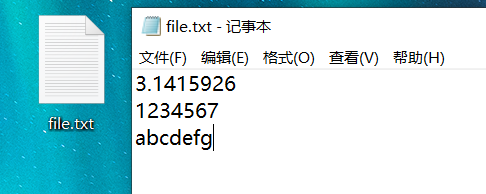
\includegraphics[width=5cm]{./figures/PyFile_1.png}
\caption{file文件内容} \label{PyFile_fig1}
\end{figure}
\begin{lstlisting}[language=matlab]
fo=open(r'C:\Users\shizy\Desktop\file.txt')
print("文件名: ", fo.name)
print("是否已关闭 : ", fo.closed)
print("访问模式 : ", fo.mode)
str = fo.read()
print(str)
fo.close()
\end{lstlisting}
输出如下
\begin{lstlisting}[language=python]
文件名:  C:\Users\shizy\Desktop\file.txt
是否已关闭 :  False
访问模式 :  r
3.1415926
1234567
abcdefg
\end{lstlisting}
上述代码第一个\verb|open|方法前面我们添加了一个\verb|r|,表示原生字符串,否则\verb|\|会对字符串进行转义处理. 当然也可以不加\verb|r|, 而使用两个\verb|\|, 效果一样. 我们在程序2-4行分别使用了文件的三种其他方法:

\verb|file.closed|	返回true如果文件已被关闭,否则返回false.

\verb|file.mode|	返回被打开文件的访问模式.

\verb|file.name|	返回文件的名称.


\textbf{write() 方法}

\verb|write()|方法可将任何字符串写入一个打开的文件.需要重点注意的是,Python字符串可以是二进制数据,而不是仅仅是文字.\verb|write()|方法不会在字符串的结尾添加换行符('\verb|\n|'). 语法如下:
\begin{lstlisting}[language=python]
fo = open("file2.txt", "wb")
fo.write( "Hello Python\n");
# 关闭打开的文件
fo.close()
\end{lstlisting}

\textbf{readline() 方法}

\verb|readline()| 会从文件中读取单独的\textbf{一行}.换行符为 '\verb|\n|'.\verb|readline()| 如果返回一个空字符串, 说明已经已经读取到最后一行.

\textbf{readlines() 方法}

\verb|readlines()| 将以列表的形式返回该文件中包含的\textbf{所有行},列表中的一项表示文件的一行.如果设置可选参数 \verb|sizehint|, 则读取指定长度的字节, 并且将这些字节按行分割.

上面介绍的文件读写方法虽然没问题,但是一般情况下我们不使用,而是使用\verb|with| 方法.从而避免忘记关闭文件导致的不可预料的结果.


\subsection{从文件中读取数据}
\subsubsection{读取整个文件}
下面的程序打开并读取这个文件, 再将其内容显示到屏幕上:
\begin{lstlisting}[language=python]
with open('file.txt') as f:
contents = f.read()
print(contents)
\end{lstlisting}
在这个程序中, 关键字\verb|with| 在不再需要访问文件后将其关闭. 在这个程序中, 注意到我们调用了\verb|open()|, 但没有调用\verb|close()|; 你也可以调用\verb|open()| 和\verb|close()| 来打开和关闭文件, 但这样做时, 如果程序存在错误, 导致\verb|close()| 语句未执行, 文件将不会关闭.  这看似微不足道, 但未妥善地关闭文件可能会导致数据丢失或受损.  如果在程序中过早地调用\verb|close()|, 你会发现需要使用文件时它已关闭, 无法访问, 这会导致更多的错误. 并非在任何情况下都能轻松确定关闭文件的恰当时机, 但通过使用前面所示的结构, 可让Python去确定: 你只管打开文件, 并在需要时使用它, Python自会在合适的时候自动将其关闭.

\subsubsection{逐行读取}
读取文件时, 常常需要检查其中的每一行: 你可能要在文件中查找特定的信息, 或者要以某种方式修改文件中的文本.
\begin{lstlisting}[language=python]
with open('file.txt') as f:
    for line in f:
        print(line)
\end{lstlisting}

利用\verb|with|来对文件的操作与上一节类似,这里不再赘述.

\subsection{数据存储}
很多程序都要求用户输入某种信息. 不管专注的是什么, 程序都把用户提供的信息存储在列表和字典等数据结构中.  用户关闭程序时, 你几乎总是要保存他们提供的信息; 一种简单的方式是使用模块\verb|json| 来存储数据.

模块\verb|json| 让你能够将简单的Python数据结构转储到文件中, 并在程序再次运行时加载该文件中的数据. 你还可以使用\verb|json| 在Python程序之间分享数据. 更重要的是, \verb|json|数据格式并非Python专用的, 这让你能够将以\verb|json|格式存储的数据与使用其他编程语言的人分享. 这是一种轻便格式, 很有用, 也易于学习.

\subsubsection{使用json.dump() 和json.load()}
我们来编写一个存储一组数字的简短程序, 再编写一个将这些数字读取到内存中的程序. 第一个程序将使用\verb|json.dump()| 来存储这组数字, 而第二个程序将使
用\verb|json.load()|.

函数\verb|json.dump()| 接受两个实参: 要存储的数据以及可用于存储数据的文件对象. 下面演示了如何使用\verb|json.dump()| 来存储数字列表.
\begin{lstlisting}[language=python]
import json
numbers = [2, 3, 5, 7, 11, 13]
filename = 'numbers.json'
with open(filename, 'w') as f_obj:
    json.dump(numbers, f_obj)
\end{lstlisting}
我们先导入模块\verb|json|, 再创建一个数字列表. 在第三行处, 我们指定了要将该数字列表存储到其中的文件的名称. 通常使用文件扩展名\verb|.json|来指出文件存储的数据为\verb|json|格式. 接下来,, 我们以写入模式打开这个文件, 让\verb|json| 能够将数据写入其中. 在第五行处, 我们使用函数\verb|json.dump()| 将数字列表存储到文件\verb|numbers.json|中.

下面再编写一个程序, 使用\verb|json.load()| 将这个列表读取到内存中:

\begin{lstlisting}[language=python]
import json
filename = 'numbers.json'
with open(filename) as f_obj:
   numbers = json.load(f_obj)
print(numbers)
\end{lstlisting}


\subsection{字符串处理}
字符串的处理个人认为在网络数据挖掘中使用非常广泛,比如网络爬虫. 对于字符串 \verb|'python String function'|, 生成字符串变量
\begin{lstlisting}[language=python]
str='python String function'
\end{lstlisting}
字符串长度获取:\verb|len(str)|
\begin{lstlisting}[language=python]
print('%s length=%d' % (str,len(str)))
\end{lstlisting}


\subsubsection{字母处理}
全部大写:\verb|str.upper()|

全部小写:\verb|str.lower()|

大小写互换:\verb|str.swapcase()|

首字母大写,其余小写:\verb|str.capitalize()|

首字母大写:\verb|str.title()|

\begin{lstlisting}[language=python]
str='python String function'
print('%s lower=%s' % (str,str.lower()))
print('%s upper=%s' % (str,str.upper()))
print('%s swapcase=%s' % (str,str.swapcase()))
print('%s capitalize=%s' % (str,str.capitalize()))
print('%s title=%s' % (str,str.title()))
输出:
python String function lower=python string function
python String function upper=PYTHON STRING FUNCTION
python String function swapcase=PYTHON sTRING FUNCTION
python String function capitalize=Python string function
python String function title=Python String Function
\end{lstlisting}
\subsubsection{格式化相关}
获取固定长度,右对齐,左边不够用空格补齐:\verb|str.ljust(width)|

获取固定长度,左对齐,右边不够用空格补齐:\verb|str.ljust(width)|

获取固定长度,中间对齐,两边不够用空格补齐:\verb|str.ljust(width)|

获取固定长度,右对齐,左边不足用0补齐

\begin{lstlisting}[language=python]
str='python String'
print('%s ljust=%s' % (str,str.ljust(20)))
print('%s rjust=%s' % (str,str.rjust(20)))
print('%s center=%s' % (str,str.center(20)))
print('%s zfill=%s' % (str,str.zfill(20)))
输出:
python String ljust=python String       
python String rjust=       python String
python String center=   python String    
python String zfill=0000000python String

\end{lstlisting}

\subsubsection{字符串搜索相关}
搜索指定字符串,没有返回-1:\verb|str.find('t')|

指定起始位置搜索:\verb|str.find('t',start)|

指定起始及结束位置搜索:\verb|str.find('t',start,end)|

从右边开始查找:\verb|str.find('t')|

搜索到多少个指定字符串:\verb|str.count('t')|

\begin{lstlisting}[language=python]
str='python String function'
print('%s find nono=%d' % (str,str.find('nono')))
print('%s find t=%d' % (str,str.find('t')))
print('%s find t from %d=%d' % (str,1,str.find('t',1)))
print('%s find t from %d to %d=%d' % (str,1,2,str.find('t',1,2)))
print('%s rfind t=%d' % (str,str.rfind('t')))
print('%s count t=%d' % (str,str.count('t')))
输出:
python String function find nono=-1
python String function find t=2
python String function find t from 1=2
python String function find t from 1 to 2=-1
python String function rfind t=18
python String function count t=3
\end{lstlisting}

\subsubsection{字符串替换相关}

替换old为new:\verb|str.replace('old','new')|

替换指定次数的old为new:\verb|str.replace('old','new',maxReplaceTimes)|


\subsubsection{字符串去空格及去指定字符}

去两边空格:\verb|str.strip()|

去左空格:\verb|str.lstrip()|

去右空格:\verb|str.rstrip()|

去两边字符串:\verb|str.strip('d')|,相应的也有\verb|lstrip,rstrip|

按指定字符分割字符串为数组:\verb|str.split(' ')|

\begin{lstlisting}[language=python]
str=' python String function '
print('%s strip=%s' % (str,str.strip()))
str='python String function'
print('%s strip=%s' % (str,str.strip('d')))
\end{lstlisting}



\subsubsection{翻转字符串}
\begin{lstlisting}[language=python]
sStr1 = 'abcdefg'
sStr1 = sStr1[::-1]
print(sStr1)
输出
gfedcba
\end{lstlisting}

\subsubsection{连接字符串}
\begin{lstlisting}[language=python]
delimiter = ','
mylist = ['Brazil', 'Russia', 'India', 'China']
print (delimiter.join(mylist))
print('abc'+'def')
输出
Brazil,Russia,India,China
abcdef
\end{lstlisting}

\subsubsection{截取字符串}
\begin{lstlisting}[language=python]
str='0123456789'
print(str[0:3]) #截取第一位到第三位的字符
print(str[:]) #截取字符串的全部字符
print(str[6:]) #截取第七个字符到结尾
print(str[:-3]) #截取从头开始到倒数第三个字符之前
print(str[2]) #截取第三个字符
print(str[-1]) #截取倒数第一个字符
print(str[::-1]) #创造一个与原字符串顺序相反的字符串
print(str[-3:-1]) #截取倒数第三位与倒数第一位之前的字符
print(str[-3:]) #截取倒数第三位到结尾
输出:
012
0123456789
6789
0123456
2
9
9876543210
78
789
\end{lstlisting}


关于更多高效的字符串处理方法,感兴趣的读者可以查阅正则表达式的使用方法.
